%
%
%
\chapter{Infinite Conductivity in Translation Invariant Systems}
\label{ch:infinite conductivity}
%
%
%
Ever since Drude published his theory about the electrical conductivity in metals \cite{Drude} at the beginning of the last century, it is well known that non-conversion of electron momentum in a system is required for finite electrical conductivity.
In Drude's model, the electrons possess a mean scattering time $\tau_{\mt{el}}$ representing the mean time between two scattering events of an electron and a lattice atom.
At each scattering event, the electrons transfer momentum to the lattice atoms, which is the reason electron momentum is not a conserved quantity.
In the case of conserved momentum, if an electrical field is exemplary applied, it accelerates electrons up to an infinite velocity, causing infinite conductivity.

In the following section, a momentum conserving system is considered and the electrical conductivity is computed using the memory-matrix-formalism, where an infinite conductivity is expected.
Beforehand, a short overview over the memory-matrix-formalism is given, followed by detailed and explicite deviations in chapter \ref{ch:memory matrix formalism}.
%
%
\section{An Overview over the Memory-Matrix-Formalsim}
\label{sec:overview MMF}
%
%
Let us assume a physical dynamical variable $\mt{A}(t)$ in an arbitrary system and an arbitrary pertubation too	.
Our interest is now the time evolution of $\mt{A}(t)$ depending on the pertubation.
Completely general, a physical dynamical variable can be splitted into two parts, a secular one and a non-secular one, which is shown in \cite{Mori}.
The latter represent processes like fluctuations or initial transient processes, which have in common a short lifetime comparing to the secular processes.
The dynamic and time evolution of $\mt{A}(t)$ is therefore dominated by secular processes.

This seperation enables a simple but clever geometrical interpretation, where dynamical variables are considered to be vectors in a vector space.
The direction of the variable $\mt{A}(t)$ is denoted as the A-axis, considering a unpertubated system in equilibrium.
Switching on a pertubation, the system is moved out of the equilibrium state and as a consequence the direction of $\mt{A}(t)$ is modified.
The projection of $\mt{A}(t)$ onto the A-axis is identified with the secular part, while the non-secular part is the part perpendicular to the projection 

First of all, the mathematical framework for this vector space has to be established.
In quantum mechanics, the Liouville space, also called as operator space, is the respective vector space of the memory-matrix-formalism.
As indicated by the name \emph{operator space}, the vectors of the Liouville space are operators, all of which being Hermitian.
The basis of the Liouville space is signified as $\{\toket{\mt{A}_{i}}\}$, where $i = 1,2,3,\dots,n$, and the corresponding dual space basis is denoted as $\{\tobra{\mt{A}_{i}}\}$.
To complete the definition of any vector space, a scalar product is required.
The following one is chosen:
%
\begin{align}
	\obraket{\mt{A}_{i}(t)}{\mt{A}_{j}(t')} = \frac{1}{\beta} \int\limits_{0}^{\beta} \dd{\lambda} \expval{\mt{A}_{i}^{\dag}(t) \mt{A}_{j}(t'+i\lambda)}.
	\label{eq:scalar product Liouville space}
\end{align}
%
The normal time evolution $\mt{A}_{i}(t) = e^{i\mt{H}t/\hbar} \mt{A}_{i}(0) e^{-i\mt{H}t/\hbar}$ of an operator should be valid so that $\mt{A}_{i}(i\lambda) = e^{-\lambda\mt{H}} \mt{A}_{i}(0) e^{\lambda\mt{H}}$ can be used.
If secular processes are neglected, the choice of the scalar product is determined under the aspect that as a consequence the time evolution of $\mt{A}(t)$ given the most probably path, see \cite{Mori}.
In quantum mechanics, the dynamic of an operator is ususally described by the Heisenberg equation of motion, which is transformed using the dyad product into the Liouville space
%
\begin{align}
	\oket{\dot{\mt{A}}_{i}(t)} = \frac{i}{\hbar} \oket{\comm{\mt{H}}{\mt{A}_{i}(t)}} = i \mt{L} \oket{\mt{A}_{i}(t)}.
	\label{eq:HEM in LS}
\end{align}
%
Here the Hermitian Liouville operator, ${\mt{L} = \hbar^{-1} \comm{\mt{H}}{\mt{\bullet}}}$, is introduced, which is defined by his action onto an arbitrary operator.
The formal solution of this equation is given by $\toket{\mt{A}_{i}(t)} = \exp(it\mt{L}) \cdot \toket{\mt{A}_{i}(0)}$, where the time evolution of an operator is therefore given by the Liouville operator.
For our approach a further operator is required in the Liouville space, namely the projection operator.
A set of arbitrary operators $\{\mt{C}_{i}\}$ is therefore defined.
The choice of them is different for each observed problem and unimportant at the moment.
The definition of the projection operator in Liouville space follows directly from the projection operator defined in the commonly used Hilbert space in quantum mechanics.
%
\begin{align}
	\mt{P} = \sum\limits_{i,j} \frac{\oket{\mt{C}_{i}(0)} \obra{\mt{C}_{j}(0)}}{\obraket{\mt{C}_{i}(0)}{\mt{C}_{j}(0)}} 
	\label{eq:projection operator}
\end{align}
%
The projection operator acting on some vector in Liouville space yields the projection onto the subspace spanned by the operator $\mt{C}_{i}$.
Thus, the operator $\mt{Q} = 1 - \mt{P}$ yields the corresponding part projected out of the subspace.
Furthermore, the projection operator is Hermitian and fullfills the two properties $\mt{P}^{2} = \mt{P}$ and $\mt{PQ} = \mt{QP} = 0$.
This completes the required mathematical basis of the memory-matrix formalism.

Correlation functions are the natural approach to describe the reaction of a dynamic variable on a pertubation.
In quantum mechanics, the correlation function is defined in Kubo's linear response theory as an integral over an expectation value of two operators, one of them being the investigated operator, and the other one being the coupling operator from the pertubation Hamiltonian.
In the Liouville space, the correlation function is defined as
%
\begin{align}
	\mathcal{C}_{ij}(t) := \obraket{\mt{A}_{i}(t)}{\mt{A}_{j}(0)} = \frac{1}{\beta} \int\limits_{0}^{\beta} \dd{\lambda} \expval{\mt{A}_{i}^{\dag}(t) \mt{A}_{j}(i\lambda\hbar)},
	\label{eq:correlation function in LS}
\end{align}
%
using the definition of the scalar product \eqref{eq:scalar product Liouville space}  in the second step.
Expressing the time evolution of $\mt{A}_{i}(t)$ with the Liouville operator, using the Laplace transformation and a few conversions yields an algebraic matrix equation of the correlation function, which has the form
%
\begin{align}
	\sum\limits_{l} \Big[\omega \delta_{il} - \Omega_{il} + i \Sigma_{il}(\omega)\Big] \mathcal{C}_{lj}(\omega) = \frac{i}{\beta} \chi_{ij}(0),
	\label{eq:algebraic equation correlation function}
\end{align}
%
where the abbreviations 
%
\begin{align}
	\Omega_{il} := i \beta \sum\limits_{k} \obraket{\dot{\mt{A}}_{i}}{\mt{C}_{k}} \chi_{kl}^{-1}(0)
	\qq{and}
	\Sigma_{il}(\omega) := i \beta \sum\limits_{k} \obra{\dot{\mt{A}}_{i}} \mt{Q} \frac{1}{\omega - \mt{QLQ}} \mt{Q} \oket{\dot{\mt{C}}_{k}} \chi_{kl}^{-1}(0)
	\label{eq:Omega&Sigma}
\end{align}
%
are introduced.
Both sums over $l$ and $k$ run over the set of operators, defined by the projection operator.
Similiarly, the indices $i$ and $j$ have to be chosen from this set of operators so that \eqref{eq:algebraic equation correlation function} yields $n^{2}$ equations, if $n$ is the number of operators in the set.
Both abbreviations can be combined to a function $M_{il}(\omega) := \Sigma_{il}(\omega) +i \Omega_{il}$, called the memory function.
In this function, $\Sigma_{il}(\omega)$ takes the role of the quantum mechanical self energy, while $\Omega_{il}$ represents dissipative effects.
$\Omega_{il}$ vanishes under to condictions.
The model Hamiltonian has to be invariant under time reversal symmetry.
Furthermore, both operators, $\mt{A}_{i}$ and $\mt{C}_{k}$, have to be the same sign with respect to time reversal symmetry.
This assertion is proven in great detail in \ref{subsec: time reversal symmetry}.
In folloes that the memory function is solely determined by $\Sigma_{il}(\omega)$.

The structur of $\Sigma_{il}(\omega)$ resembles the one of the Laplace transformed correlation function, comparing equation \eqref{eq:correlation function frequency space}, with two differences.
The expectation value is performed with respect to the operators like $\mt{Q}\toket{\dot{\mt{A}}_{i}}$ instead of $\toket{\mt{A}_{i}}$, while only the reduced Liouville operator QLQ is considered.
The latter projects at the part of the full Liouville operator, which causes the intrinsic fluctuations of the operator $\mt{A}$.
In other words, the operator QLQ describes the internal dynamics of all other degrees of freedom of the system, called the \emph{bath}, excluded A.
The coupling to the bath is characterizied by the vector $\mt{Q}\toket{\dot{\mt{A}}_{i}}$ and is clearly changing the dynamic behaviour of A.
%
%
\section{Electrical Conductivity in a Momentum Conserving System}
\label{sec:conductivity conserved momentum}
%
%
%
\begin{figure}[t]
	\centering
	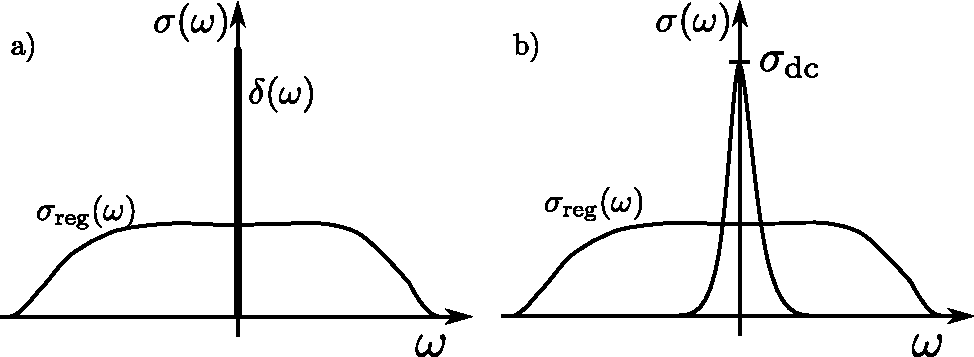
\includegraphics[width=0.9\textwidth]{conductivity.pdf}
	%\subfigure[infinite conductivity considering unbroken translation symmetry]{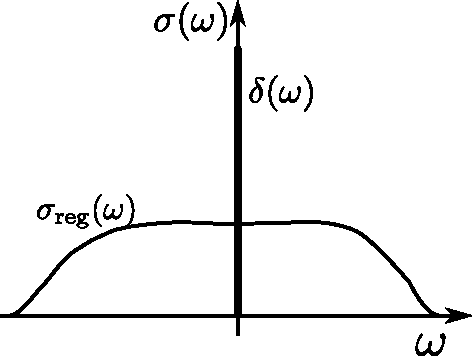
\includegraphics[width=0.45\textwidth]{conductivity_delta_peak.pdf}}
	%\subfigure[finite conductivity considering broken translation symmetry]{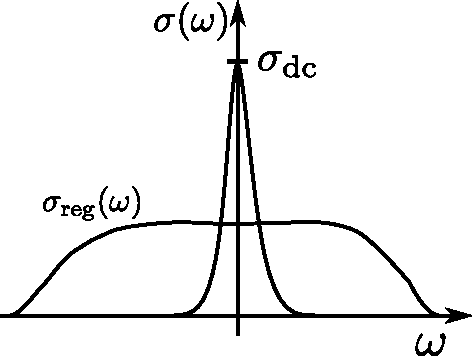
\includegraphics[width=0.45\textwidth]{conductivity_drude_peak.pdf}}
	\caption{
Figure a) and b) shown the static electrical conductivity in a un-pertubated and pertubated system, respectively.
In a system with unbroken translation symmetry, the relaxation of momentum is impossible to other degrees of freedom. 
As a consequence, the static conductivity is infinite. This is illustrated in a).
Switching on a pertubation as umklapp scattering, the translation symmetry is broken.
The static conductivity becomes finite due to the relaxation of momentum to other degrees of freedom.
In both figures, the regular conductivity, caused by fluctuation e.\,g., is denoted as $\sigma_{\mt{dc}}$.
	}
	\label{fig:conductivity broken and unbroken translation symmetry}
\end{figure}
%
In the following section, the electrical conductivity is computed for a system, where momentum is conserved, using the memory-matrix-formalism.
An infinite conductivity is expected due to the fact that electrons do not transfer any momentum to other degrees of freedom.
Besides conserving momentum, the observed system has to satisfy some additional requirements.
Firstly, the current has to be an unconserved quantitiy.
Furthermore, the scalar product $\tobraket{\mt{J}}{\mt{P}}$ of current and momentum has to be non-zero.
In other words, both quantities possess a finite overlap.
These two quantities should also generate the subspace into the projection operator projects.
The sum in \eqref{eq:projection operator} summerizes over all operators $\mt{C}_{i}$, where the choice has now to be done with respect to the electrical conductivity.
As electrical conductivity is determined by momentum and current, these are chosen as operators.
The last requirement is for the Hamiltonian to be invariant under time reversal symmetry, which is our last requirement.

Nevertheless, one remark has to be made for computing the conductivity.
Due to the fact that the Hamiltonian is invariant under time reversal symmetry and the subspace is generated by J and P, which have same signature under time reversal symmetry, no dissipative effects exist.
The quantity $\Omega$, defined in \eqref{eq:Omega&Sigma}, is therefore zero.

In the strictly general sense, the electrical conductivity is given by the current-current correlation function $\mathcal{C}_{\mt{JJ}}(\omega)$ (see \cite{Chycholl2}).
The static case is obtained by taking the small frequency limit, $\omega \to 0$, of the conductivity.
%
\begin{align}
	\sigma_{\mt{dc}} = \lim\limits_{\omega \to 0} \sigma(\omega) = \lim\limits_{\omega \to 0}\, \beta\,\mathcal{C}_{\mt{JJ}}(\omega)
	\label{eq:general static condictivity}
\end{align}
%
The current-current correlation function is given by equation \eqref{eq:algebraic equation correlation function}, which is in the case of the J-P subspace a $2\times2$ matrix equation.
The quantity $\Sigma$ is simplified by two aspects.
Firstly, the momentum is conserved, which means the time derivative of P is zero and therefore all expectation values are trivially zero where $\dot{\mt{P}}$ is a taken vector.
The remaining expectation values of $\Sigma$ contains only the current J, but these ones are vanishing as well.
The operator QLQ describes the intrinsic fluctuation of $\toket{\mt{J}}$, which are assumed to be zero.
Furthermore, the operator Q acting on $\toket{\mt{J}}$ yields the coupling to these intrinsic fluctuation and, leading to $\mt{Q}\toket{\mt{J}} = 0$.
The obtained matrix equation has a very simple form and the current-current correlation function can be directly read out as
%
\begin{align}
	\mathcal{C}_{\mt{JJ}}(z) = \frac{i}{\omega} \beta^{-1} \chi_{\mt{JJ}}(\omega=0) = \frac{i}{\omega} \mathcal{C}_{\mt{JJ}}(t=0),
	\label{eq:correlation function unpertubated system}
\end{align}
%
where relation \eqref{eq:relation between C, Phi and chi} is being used.
The correlation function at time $t = 0$ is given by the scalar product $\tobraket{\mt{J}(0)}{\mt{J}(0)}$ (see \eqref{eq:correlation function in LS}).
Due to the fact that current and momentum are two closely connected quantities, this is also valid for their correlation functions
For this reason, the current-current correlation function is expresed with respect to the momentum-momentum correlation function.

The vector operator $\toket{\mt{J}(0)}$ is seperated into two pieces, one parallel and one perpendicular part, which are labeled as $\oket{\mt{J}_{\mid\mid}}$ and $\oket{\mt{J}_{\bot}}$, respectivily.
As discussed above, every variable generally consists of a secular and non-secular part, which does not mean that both parts need to exist in the observing model.
The non-secular part is represented by the perpendicular component of $\toket{J}$.
In the experiement, these processes are obseved as a constant slowly fluctuating background, known as noise.
The secular part is represented by the parallel component of $\toket{J}$, which is responsible for the electrical condictivity and is visable as a peak in the measurement, depicted in figure \ref{fig:conductivity broken and unbroken translation symmetry}.

Drude's theory of conductivity yields a direct proportionality between J and P (see for example \cite{Gross&Marx}).
Since momentum is conserved and current is unconserved, in the investigated system this proportionality can't be valid.
Nevertheless, both quantities possess a finite overlap, which means that a part of the current is conserved and therefore parallel to the momentum.
This part is the parallel component of J and given by the projection von $\toket{\mt{J}}$ onto $\toket{\mt{P}}$.
%
\begin{align}
	\oket{\mt{J}_{\mid\mid}} = \mathcal{P}\oket{\mt{J}} = \frac{\odyad{\mt{P}}{\mt{P}}}{\obraket{\mt{P}}{\mt{P}}} \oket{\mt{J}} = \frac{\chi_{\mt{PJ}}}{\chi_{\mt{PP}}} \oket{\mt{P}}
	\label{eq:parallel current as projection}
\end{align}
%
Seperating both current operator in $\tobraket{\mt{J}(0)}{\mt{J}(0)}$ yields four new correlation functions, where the mixed ones are zero, since $\oket{\mt{J}_{\mid\mid}}$ and $\oket{\mt{J}_{\bot}}$ are perpendicular to each other by construction.
For the operators in the parallel correlation function, $\tobraket{\mt{J}_{\mid\mid}(0)}{\mt{J}_{\mid\mid}(0)}$ equation \eqref{eq:parallel current as projection} is used.
In this equation, the correlation function of the parallel components is represented as a momentum-momentum correlation function.
Inserting the obtained expression for the current-current correlation function in \eqref{eq:correlation function unpertubated system} the conductivity is given by 
%
\begin{align}
	\sigma (\omega) = \frac{\vert\chi_{\mt{PJ}}\vert^{2}}{\vert\chi_{\mt{PP}}\vert} \frac{i}{\omega}  + \sigma_{\mt{reg}}(\omega),
\end{align}
%
where the momentum-momentum correlation function is expressed as static susceptibility (see \eqref{eq:relation between C, Phi and chi}), and the regular conductivity $\sigma_{\mt{reg}}(\omega) = i(\omega \beta)^{-1} \tobraket{\mt{J}_{\bot}}{\mt{J}_{\bot}}$ is introduced, which representes the noise (see figure \ref{fig:conductivity broken and unbroken translation symmetry}).

In the above equation the quantity $\omega$ is a complex number.
Since $\omega$ has to be a real number for a physical interpetation, it is transformed on the real axis using analytical continuation.
The conductivity is then given by
%
\begin{align}
	\sigma(\omega) = \frac{\vert\chi_{\mt{PJ}}\vert^{2}}{\vert\chi_{\mt{PP}}\vert} \bigg(\PV{\frac{i}{\omega}} + \pi \delta(\omega) \bigg) + \sigma_{\mt{reg}}(\omega)
	\label{eq:conductivity unpertubed system}
\end{align}
%
where $\frac{1}{\omega + i\eta} = \PV{\frac{1}{\omega}} - i\pi\delta(\omega)$ is used and $\PV$ symbolizies the prinzipel value.
Taking now the small frequency limit $\omega \to 0$ the $\delta$-distribution is the dominant term and the static conductivity becomes infinite, which is the exactly expected result.
The static electrical conductivity is infinite in a momentum conserving system, thus conductivity is getting finite if the momentum is not a conserved quantity any more.
The respective underlying symmetry is translation symmetry.
For breaking this symmerty, many possibilities are available, but in the following computation only one of them, namely umklapp scattering, is considered.

In the next chapter, the observed spin-fermion model is introduced.
Beforehand, quantum phase transitions are reviewed.
The conservation of momentum and non-conversation of current is further constituted.
Finally, umklapp scattering is introduced for breaking translation symmetry and unconserving momentum.
























